\documentclass{article}
\usepackage{amsmath,amsthm,amssymb,amsfonts}
\usepackage{setspace,enumitem}
\usepackage{graphicx}
\usepackage{hyperref}
\usepackage{natbib}
\usepackage{afterpage}
\usepackage{xcolor}
\usepackage{etoolbox}
\usepackage{booktabs}
\usepackage{pdfpages}
\usepackage{multicol}
\usepackage{geometry}
\usepackage{bbm}
\usepackage{csvsimple}
\usepackage{accents}
\hypersetup{
	colorlinks,
	linkcolor={blue!90!black},
	citecolor={red!90!black},
	urlcolor={blue!90!black}
}

\newtheorem{theorem}{Theorem}
\newtheorem{assumption}{Assumption}
\newtheorem{definition}{Definition}
\newtheorem{lemma}{Lemma}
\setlength{\parindent}{0cm}
\geometry{margin = 1in}

\newcommand{\R}{\mathbb{R}}
\newcommand{\ubar}[1]{\underaccent{\bar}{#1}}
\newcommand{\F}{\mathcal{F}}
\newcommand{\xbf}{\mathbf{x}}
\newcommand{\Xbf}{\mathbf{X}}
\newcommand{\Vbf}{\mathbf{V}}
\newcommand{\zbf}{\mathbf{z}}
\newcommand{\Tbf}{\mathbf{T}}
\newcommand{\mubf}{\boldsymbol{\mu}}
\newcommand{\alphabf}{\boldsymbol{\alpha}}
\newcommand{\betabf}{\boldsymbol{\beta}}
\newcommand{\sigmabf}{\boldsymbol{\sigma}}
\newcommand{\onebf}{\mathbbm{1}}
\newcommand{\Covbf}{\text{\textbf{Cov}}}
\newcommand{\Varbf}{\text{\textbf{Var}}}

\newtoggle{extended}
\settoggle{extended}{false}

\title{ECON 899B: Besanko and Doraszelski Replication}

\author{Alex von Hafften}

\begin{document}

\maketitle

Here, I replicate Besanko and Doraszelski (2004).  I run the model for quantity and price competition for $\delta = 0.1$ and $\delta =0.3$. There are three Julia files:

\begin{itemize}

\item model.jl contains the code to estimate the model.

\item plotting.jl contains the code to make plots.

\item run.jl runs the model with different parameterizations.

\end{itemize}

In this write-up, I plot the static results (i.e. the quantity decisions, the pricing decisions, and the profit) and the dynamic results (i.e. the investment decisions, the franchise value, and the stationary distribution) for each parameterization of the model.

\bigskip

Besanko and Doraszelski have four levels of depreciation $\{0.0, 0.01, 0.1, 0.3\}$, but I ran into issues with both the firm problem and the stationary distribution converging, so I opted to focused on the relatively higher depreciation levels.  I tried to compute the stationary distribution instead of focusing on the distribution a number of periods in the future like Besanko and Doraszelski (mostly by accident).  It would have probably been better to just think of the distribution $T$ into the future.

\pagebreak

\section*{Static Results}

Below are the static results for the quantity competition.  These are the same across levels of depreciation.  The optimal quantity, price, and profit are the rows and the columns are firm 1 and firm 2.  The problem is symmetric so firm 1's results are the transpose of firm 2's results.

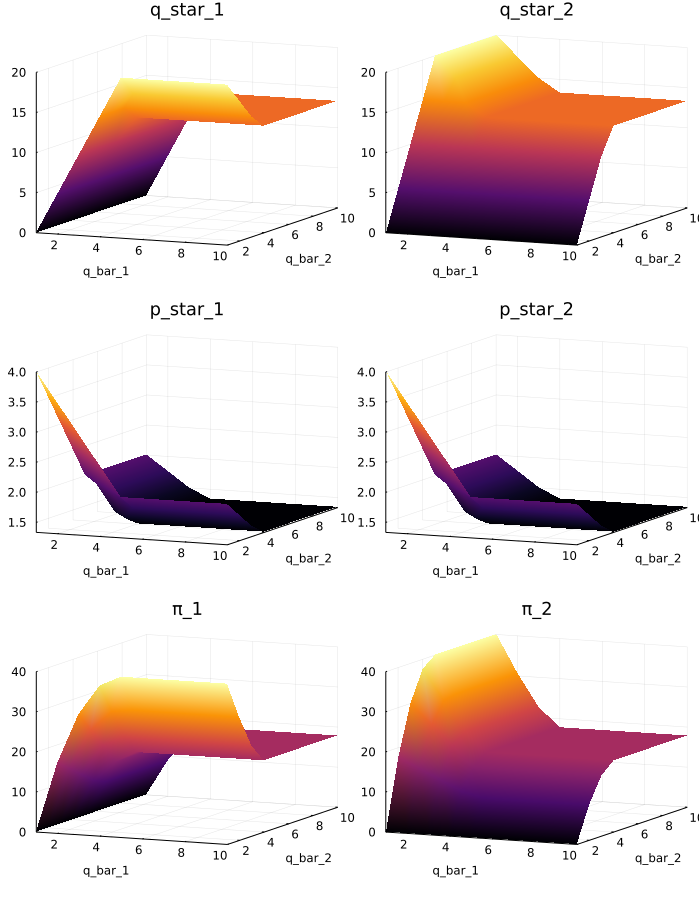
\includegraphics[scale=.65]{q_static.png}

\pagebreak

Below are the static results for the price competition.  This is generally more involved than the quantity competition because there are different cases to consider. See the paper and the code for more details.  The most striking result here is the typical Bertand case that if both firms are large prices go to marginal cost and profit is zero.

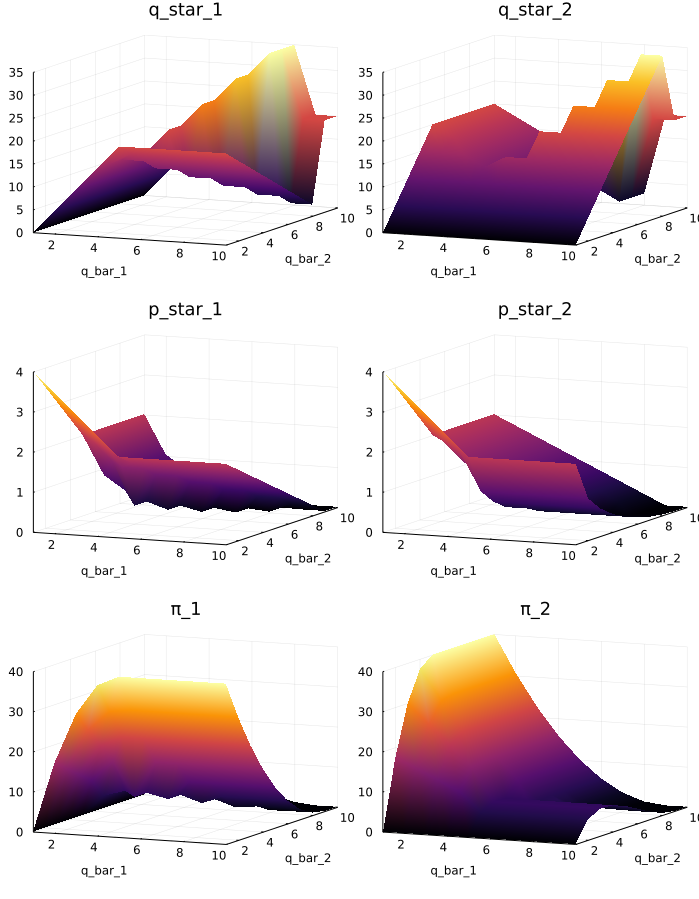
\includegraphics[scale=.65]{p_static.png}

\pagebreak

\section*{Dynamic Results}

Below are the dynamic results for quantity competition with a relatively low delta ($\delta = 0.1$).  The rows are the investment policy function, the franchise value, and the stationary distribution.  The first column is for firm 1 and the second column is for firm 2.

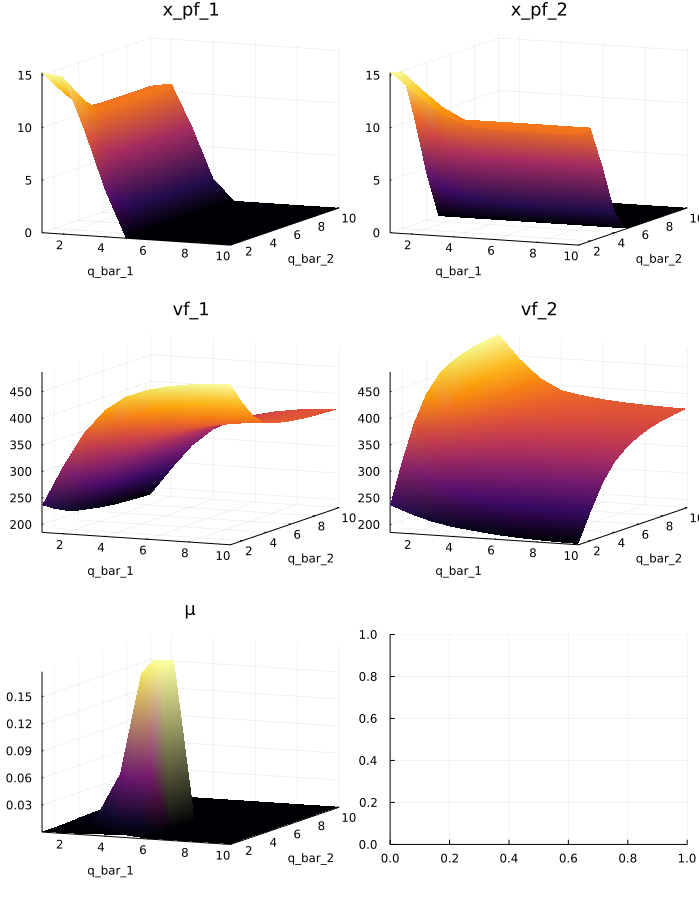
\includegraphics[scale=.65]{q_low_delta_dynamic.png}

\pagebreak

Below are the dynamic results for quantity competition with a relatively high delta ($\delta = 0.3$). We can clearly see how the stationary distribution is ``flatten" out.

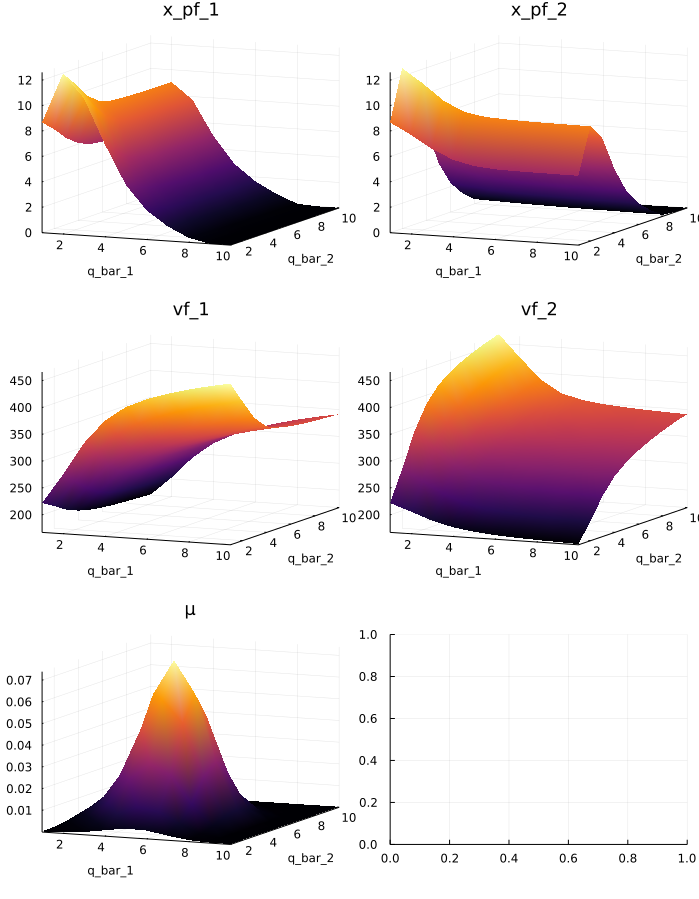
\includegraphics[scale=.65]{q_high_delta_dynamic.png}

\pagebreak

Below are the dynamic results for price competition with a relatively low delta ($\delta = 0.1$). The stationary distribution shows the one-large-firm-and-the-one-small-firm result from Besanko and Doraszelski.

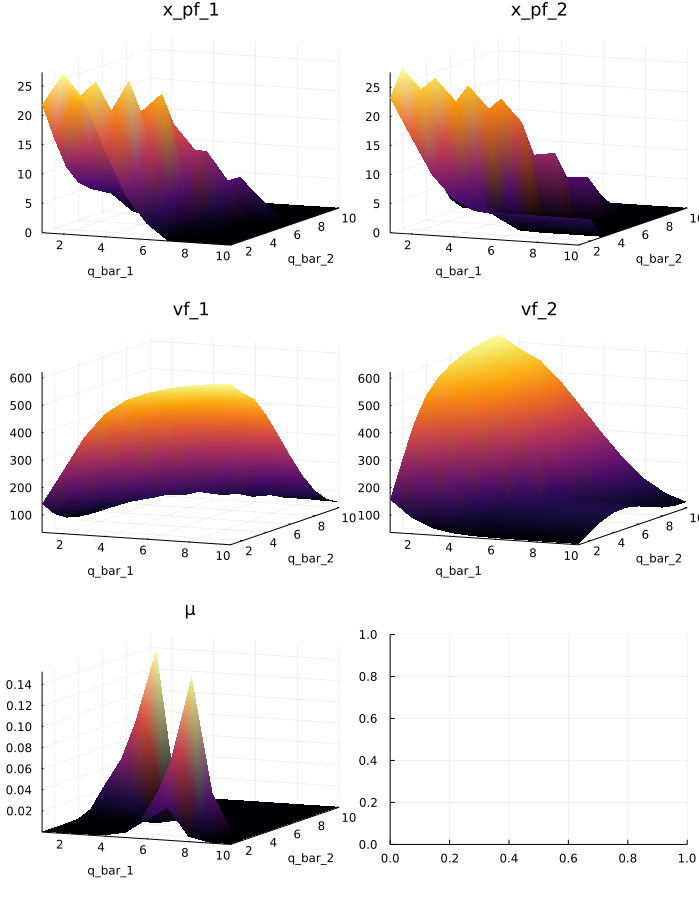
\includegraphics[scale=.65]{p_low_delta_dynamic.png}

\pagebreak

Below are the dynamic results for price competition with a relatively high delta ($\delta = 0.3$). The higher depreciation rate merged the two humps.  I'm not quite sure what to make of this distribution because it is no longer symmetric.

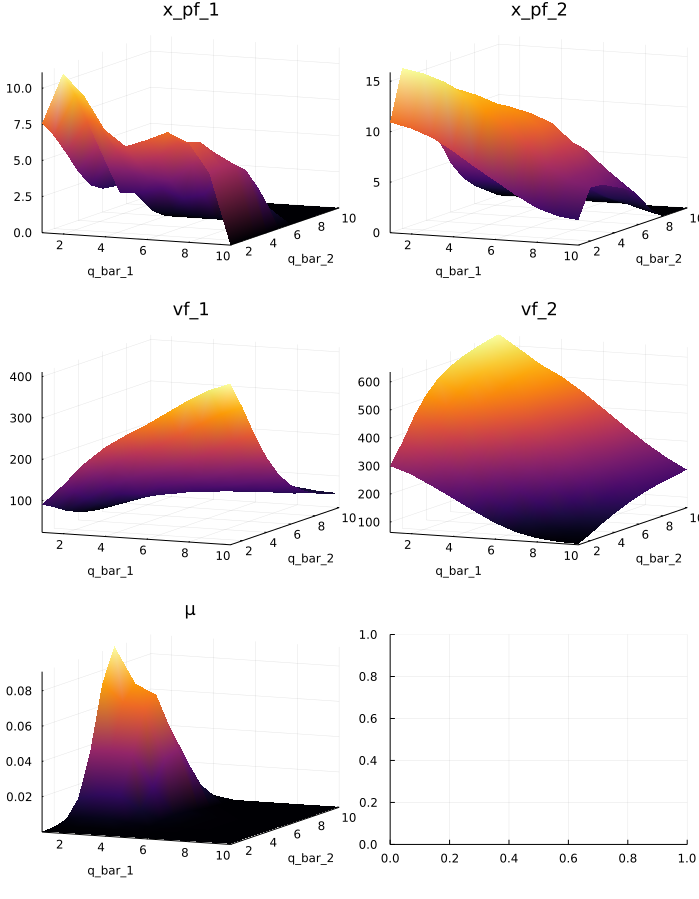
\includegraphics[scale=.65]{p_high_delta_dynamic.png}


\end{document}

